\documentclass[final]{beamer}

% Font and Encoding
\usepackage[T1]{fontenc}
\usepackage{lmodern}
\usepackage{anyfontsize}

% Beamerposter and Theme Configuration
\usepackage[orientation=portrait,size=a0,scale=1.15]{beamerposter}
\usetheme{gemini}
\usecolortheme{nott}

% Modern Package Set for Academic Rigor
\usepackage{amsmath}
\usepackage{amssymb}
\usepackage{graphicx}
\usepackage{booktabs}
\usepackage{microtype}
\usepackage{csquotes}
\usepackage[backend=biber,style=numeric]{biblatex}
\usepackage{tikz}
\usepackage{pgfplots}
\usepackage[dvipsnames]{xcolor}
\pgfplotsset{compat=1.14}
\usepackage[version=4]{mhchem}


% Hyperref and Cleveref must be loaded last
\usepackage{hyperref}
\usepackage{cleveref}

% Ensure 3cm lateral margins for the main text blocks
\setbeamersize{text margin left=3cm,text margin right=3cm}
\setbeamertemplate{navigation symbols}{}

% Document Metadata
\title{Nanopartículas de Plata (AgNPs): \\ Síntesis Biogénica y Óptica No Lineal}
\author{Julian L. Avila-Martinez}
\institute{Física - Universidad Distrital Francisco Jose de Caldas}
\newcommand{\email}{jlavilam@udistrital.edu.co}

% Upper Header Template
\setbeamertemplate{headline}{
  \begin{tikzpicture}[x=1cm, y=1cm]
    % Tensor vertical expandido a 17cm
    \useasboundingbox (0,0) rectangle (\paperwidth, 17);
    % Dominio del título ampliado a 12.5cm
    \fill[headline.bg] (0,0) rectangle (\paperwidth, 12.5);
    \fill[white] (0, 12.5) rectangle (\paperwidth, 17);

    % Logo retornado a la izquierda (north west), ajustado en el nuevo eje Y y escalado
    \node[anchor=north west, inner sep=0pt] at (3, 16.8) {
      
\includegraphics[height=4.2cm]{./figures/logo-upper.pdf}
    };

    \node[anchor=north, align=center, text=black] at (\paperwidth/2, 16.2) {
      \Large Encuentro de Socialización de Posters en Ciencia de \\[0.3cm]
      \Large Materiales y Nanotecnología 2026-1
    };

    % Nodo de título recalibrado al centro exacto del área naranja (12.5 / 2 = 6.25)
    \node[anchor=center, align=center, text=white, text width=0.9\paperwidth] at (\paperwidth/2, 6.25) {
      {\fontsize{70}{85}\selectfont \spaceskip=0.4em \textbf{\inserttitle} \par}
      \vspace{0.6cm}
      {\Large \insertauthor \par}
      \vspace{0.25cm}
      {\normalsize \insertinstitute \par}
      \vspace{0.25cm}
      {\normalsize \texttt{\email} \par}
    };
  \end{tikzpicture}
}

% Lower 18cm Footer Template
\setbeamertemplate{footline}{
  \rule{0pt}{18cm} % Ensures background remains strictly canvas white
  \usebeamercolor{headline} % Extracts the exact purple color for TikZ
  \begin{tikzpicture}[remember picture, overlay]
    % Define fundamental anchor points along the central horizontal axis
    \coordinate (bot-left) at
      ([xshift=3cm, yshift=8cm]current page.south west);
    \coordinate (bot-right) at
      ([xshift=-3cm, yshift=8cm]current page.south east);
    \coordinate (bot-center) at
      ([yshift=8cm]current page.south);

    % Left university logo anchored to the west
    \node[anchor=west, inner sep=0pt] at (bot-left) {
      
\includegraphics[height=10cm]{./figures/logo-ud-ver.pdf}
    };

    % Center academic program box anchored to the center
    \node[anchor=center, inner sep=1cm, fill=headline.bg,
          rounded corners=1.5cm, minimum width=0.5\paperwidth,
          minimum height=8cm, align=center, text width=0.40\paperwidth,
          text=white, font=\bfseries] at (bot-center) {
      \Large Programa Académico de Física \\[0.5cm]
      \Large Facultad de Ciencias Matemáticas y Naturales
    };

  \usebeamercolor{headline}
  \node[
    anchor=east,
    fill=bg,
    text=white,
    rounded corners=0.5cm,
    inner sep=0.5cm,
    align=center
    ] at (bot-right) {
      {\large Referencias} \\[0.3cm]
      
\includegraphics[width=8cm, height=8cm, keepaspectratio]{./figures/qr-bib.pdf}
    };

\end{tikzpicture}
}

\begin{document}
\begin{frame}[t]

  \begin{block}{Resumen}
    El confinamiento a nanoescala en nanopartículas de plata (AgNPs) origina
    propiedades optofísicas emergentes dictadas por la resonancia de plasmón de
    superficie localizado (LSPR). Esta revisión estructura el conocimiento
    reciente (2020--2026) sobre la síntesis biogénica, la dinámica de la LSPR y
    la consecuente respuesta óptica no lineal. Se evidencia el rol fundamental
    de la biocorona en la sintonización plasmónica y en la estabilización de
    matrices complejas. Bajo campos intensos, el confinamiento local amplifica
    la susceptibilidad de tercer orden, posibilitando mecanismos de absorción
    inversa saturable (RSA). La literatura indica que superar la estocasticidad
    bioquímica y el amortiguamiento plasmónico resulta imperativo para
    desarrollar modelos teóricos unificados y dispositivos optoelectrónicos
    viables.

    \smallskip
    \textbf{Palabras clave:} Nanopartículas de plata, resonancia de plasmón
    de superficie localizado, óptica no lineal, síntesis biogénica,
    absorción inversa saturable.
  \end{block}

  \vspace{-1.cm}

  \begin{columns}[t]
    \begin{column}{0.48\textwidth}

      \begin{block}{Introducción}
        El confinamiento espacial de la materia a la nanoescala rompe la
        simetría traslacional del volumen, originando la resonancia de plasmón
        de superficie localizado (LSPR). Esta dinámica electrónica coherente
        rige la electrodinámica de las AgNPs. Bajo campos electromagnéticos
        intensos, el confinamiento local amplifica severamente la
        susceptibilidad óptica no lineal. El propósito de este trabajo es
        sintetizar y estructurar la literatura fundamental sobre síntesis
        sostenible, teoría plasmónica y respuesta no lineal.
      \end{block}

      \begin{block}{Metodología}
        Se ejecutó una revisión sistemática en Scopus, ScienceDirect, Web of
        Science, SpringerLink y Google Scholar abarcando el lapso 2020--2026.
        La exploración booleana inicial identificó más de 10 000 registros. Un
        filtrado riguroso, que excluyó estudios restringidos a óptica lineal,
        destiló un corpus final de 43 artículos experimentales y teóricos.
      \end{block}

      \begin{block}{Naturaleza de las AgNPs}
        Las nanopartículas de plata (AgNPs) constituyen sistemas mesoscópicos
        formados por agregados de plata elemental con dimensiones críticas en el
        rango de 1 a 100 nanómetros. El confinamiento espacial de los electrones
        de conducción en estas geometrías altera la función de respuesta
        dieléctrica respecto al material masivo. Esta reducción dimensional
        determina la aparición de la resonancia de plasmón de superficie
        localizado (LSPR), un fenómeno electrodinámico colectivo donde la
        densidad de carga electrónica oscila de forma coherente en fase con un
        campo electromagnético excitador.
      \end{block}

      \begin{block}{Resultados Bibliométricos}

        \vspace{-0.5cm}

        \begin{figure}[htbp]
          \centering
          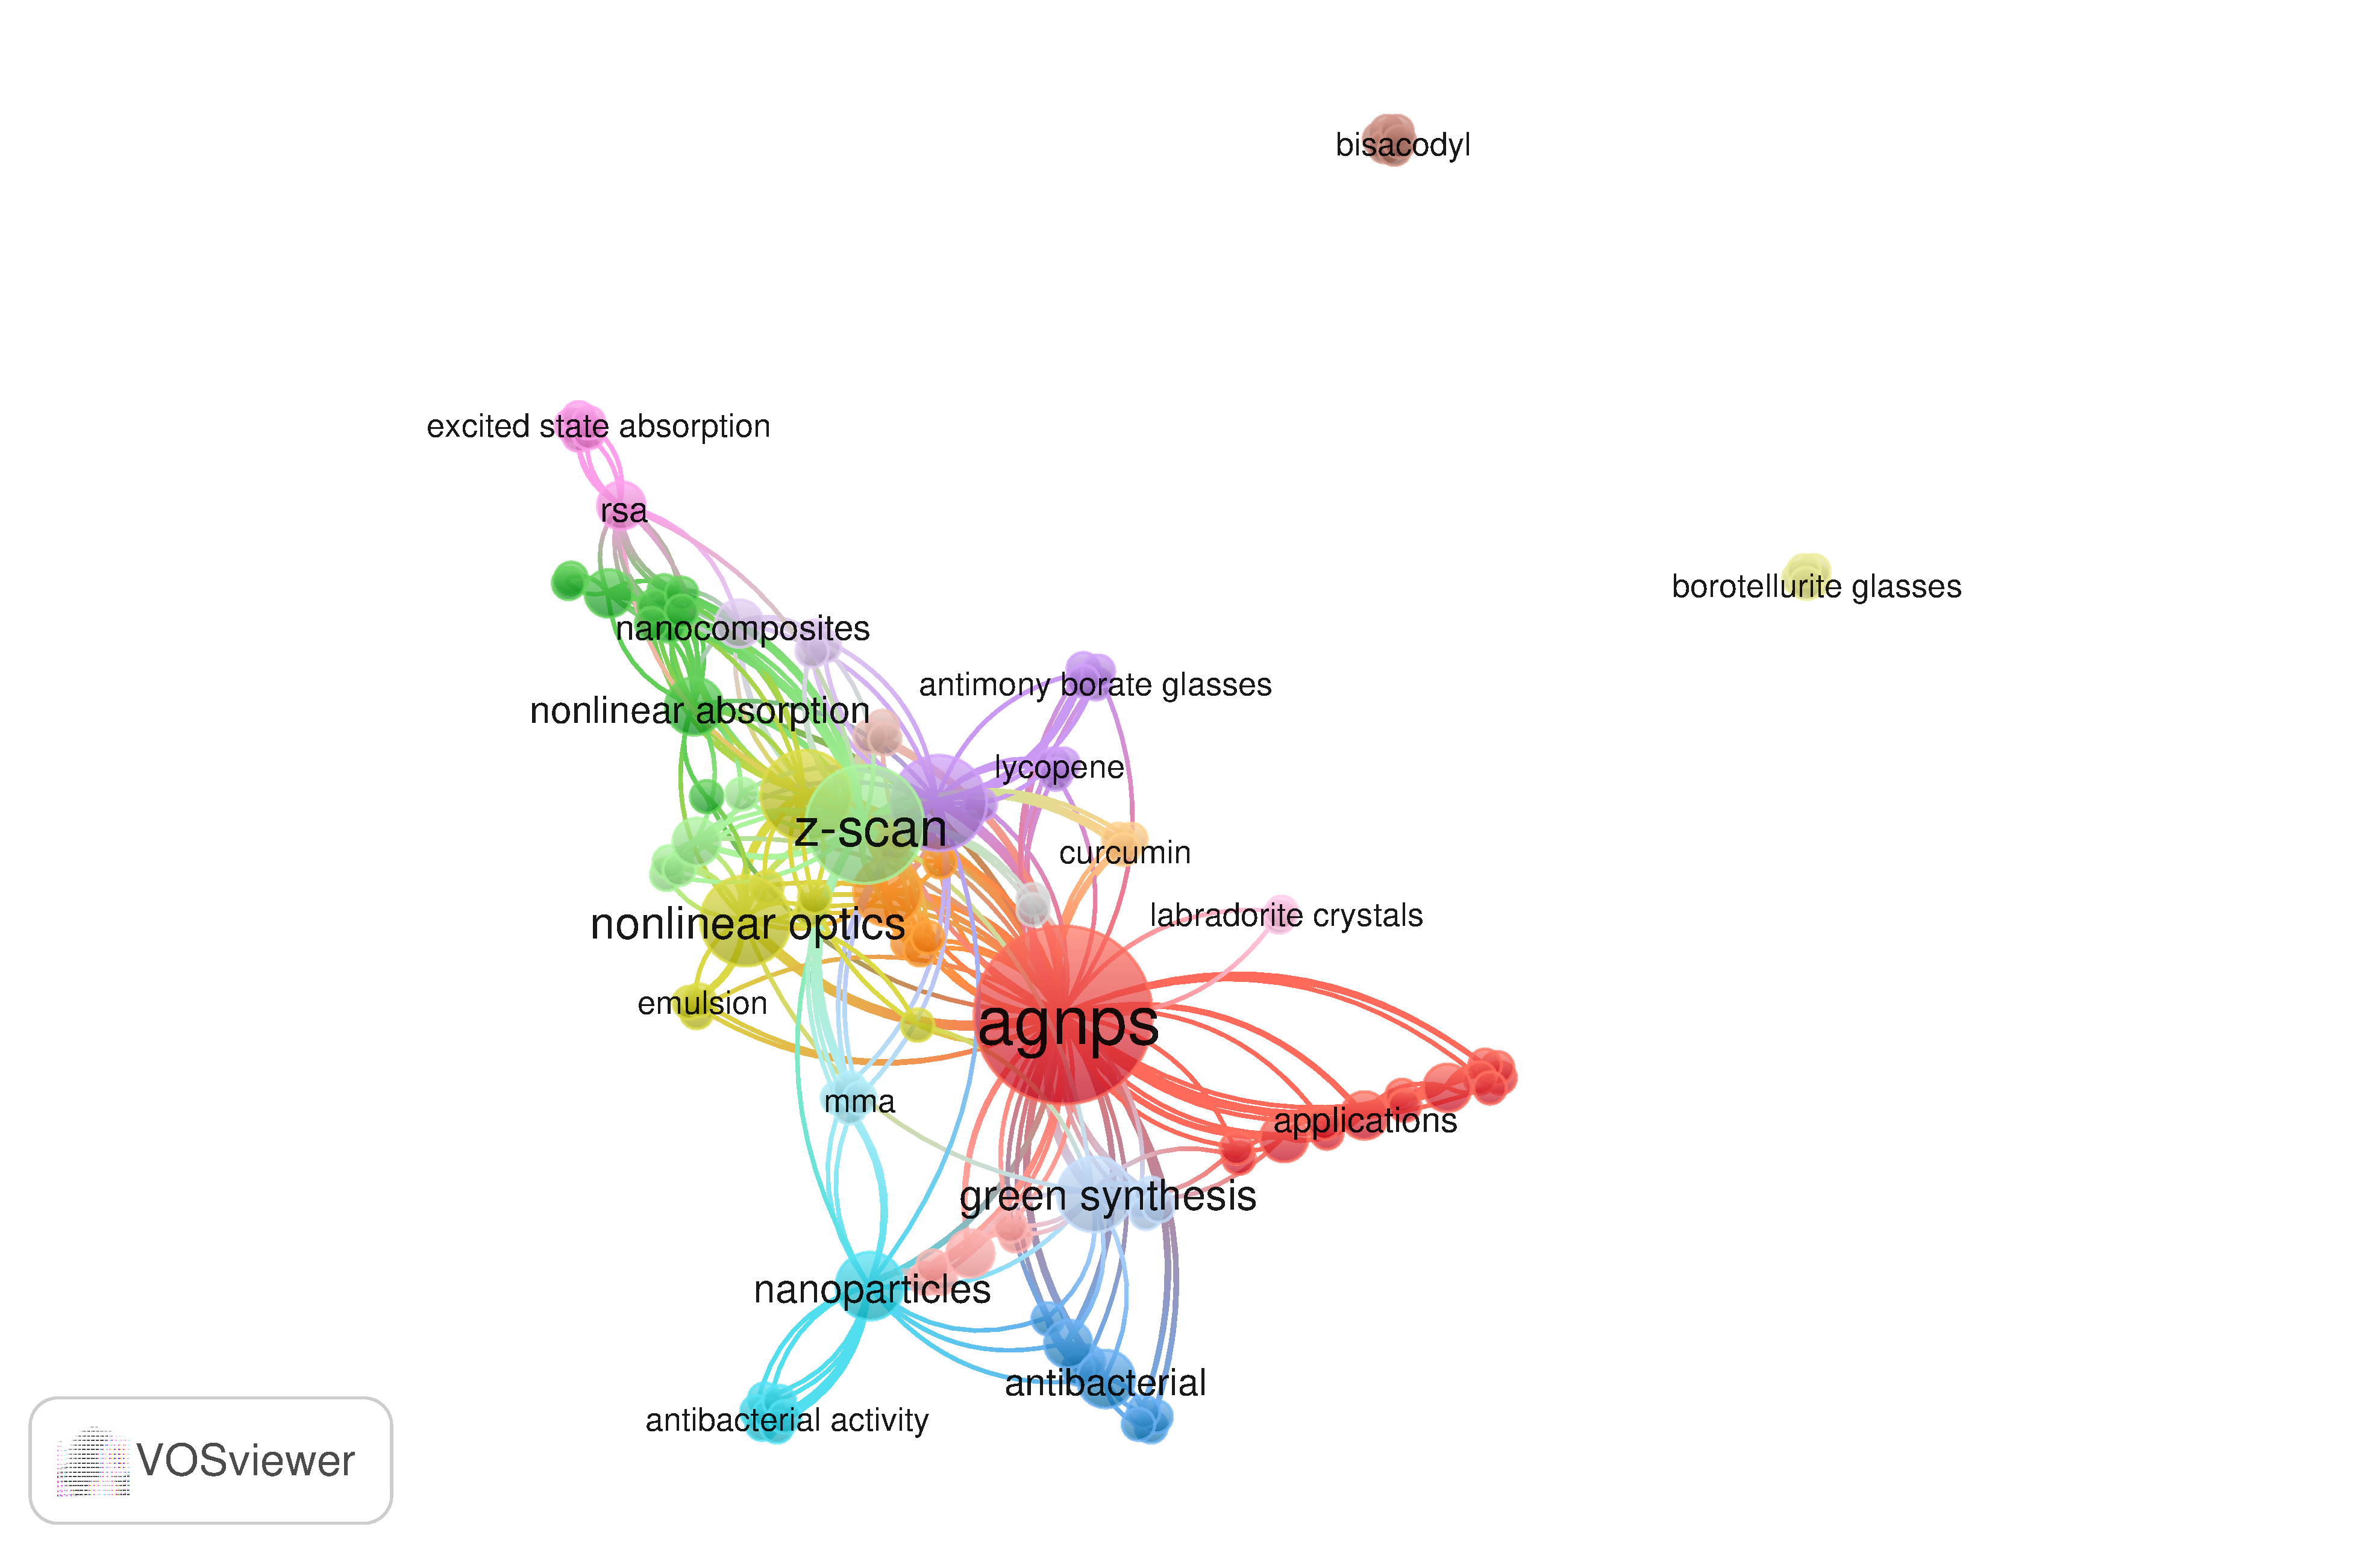
\includegraphics[width=0.9\textwidth]{../document/key-word-map.pdf}
          \caption{Mapa de coocurrencia de palabras clave. Se identifican
          clústeres de síntesis verde y caracterización óptica.}
        \end{figure}

        \vspace{-1.5cm}

        \begin{figure}[htbp!]
          \centering
          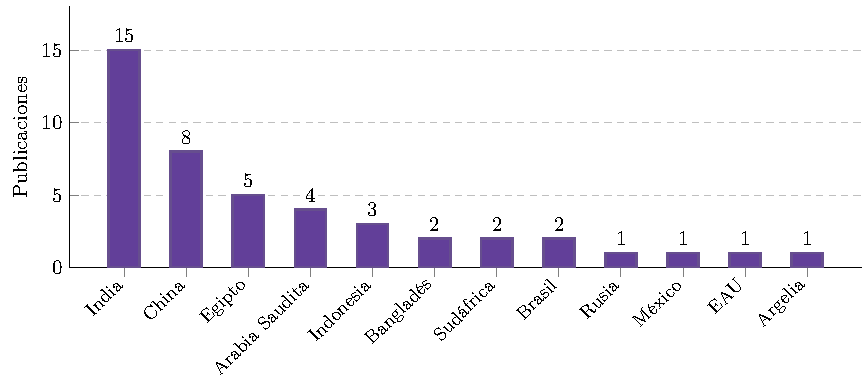
\includegraphics[height=12cm, width=0.9\textwidth, keepaspectratio]{./figures/barr.pdf}
          \vspace{-1.5cm}
          \caption{Distribución geográfica destacando el liderazgo del Sur Global.}
        \end{figure}
      \end{block}
    \end{column}

    \begin{column}{0.48\textwidth}
      \begin{itemize}
        \item La red de palabras clave bifurca el campo de estudio entre la
          física fundamental (escaneo Z, óptica no lineal) y la ciencia de
          biomateriales.
        \item El análisis de afiliaciones muestra una concentración
          investigativa predominante en el Sur Global.
        \item La investigación experimental está liderada de forma significativa
          por India, China y Egipto.
      \end{itemize}
      \begin{block}{Síntesis Biogénica y Verde}
        \begin{itemize}
          \item Transición termodinámica desde rutas químicas hacia métodos
            biogénicos para omitir precursores tóxicos.
          \item Extractos naturales proveen fitocompuestos que actúan de manera
            simultánea como reductores de iones $\ce{Ag^+}$ y agentes
            pasivantes.
          \item Se conforma una biocorona estabilizadora que redefine
            las condiciones dieléctricas locales y sintoniza la LSPR.
          \item Este paradigma biogénico introduce el concepto de toxicología
            verde; la alta estabilidad en matrices complejas es crítica para
            prevenir la bioacumulación.
        \end{itemize}
      \end{block}

      \begin{block}{LSPR y Óptica No Lineal}
        La LSPR consiste en una oscilación electrónica coherente impulsada por
        la interacción de Coulomb. En la aproximación cuasiestática de Mie,
        la polarizabilidad $\alpha$ se expresa como
        \begin{equation}
          \alpha = 4\pi R^3
          \frac{\varepsilon_m(\omega) - \varepsilon_d}
          {\varepsilon_m(\omega) + 2\varepsilon_d}.
        \end{equation}
        La resonancia emerge bajo la condición de Fröhlich,
        $\varepsilon_1(\omega) \to -2\varepsilon_d$. Bajo irradiación intensa,
        la polarización macroscópica inducida $P_i$ exige una expansión del
        tensor de susceptibilidad
        \begin{equation}
          P_i = \varepsilon_0 \left( \sum_j \chi_{ij}^{(1)} E_j + \dots +
          \sum_{j,k,l} \chi_{ijkl}^{(3)} E_j E_k E_l \right).
        \end{equation}
        El confinamiento plasmónico amplifica el tensor de tercer orden
        $\chi_{ijkl}^{(3)}$. Evaluadas mediante la técnica de escaneo Z,
        las AgNPs exhiben dinámicas de absorción transitorias dependientes
        de la fluencia del campo.

        \vspace{1cm}
        \begin{figure}[htbp!]
          \centering
          \begin{tikzpicture}[scale=1.2, transform shape, thick]
            \draw (0,0) -- (4,0) node[right] {$S_0$ (Estado Fundamental)};
            \draw (0,2) -- (4,2) node[right] {$S_1$ (Primer Estado Excitado)};
            \draw (0,4) -- (4,4) node[right] {$S_2$ (Segundo Estado Excitado)};
            \draw[->, blue] (0.8,0) -- (0.8,2);
            \node[blue, left] at (0.8,1) {SA};
            \draw[->, gray, dashed] (1.4,2) -- (1.4,0);
            \node[gray, right] at (1.4,1) {\small Blanqueamiento};
            \draw[->, red] (3.0,2) -- (3.0,4);
            \node[red, left] at (3.0,3) {RSA (ESA)};
          \end{tikzpicture}
        \end{figure}
        \vspace{0.5cm}

        La absorción inversa saturable (RSA) constituye el mecanismo pasivo
        fundamental para la limitación óptica en sensores optoelectrónicos.
      \end{block}

      \begin{alertblock}{Conclusiones}
        Las AgNPs representan un sistema físico riguroso para la integración de
        la plasmónica y la nanobiotecnología. La explotación tecnológica
        enfrenta limitaciones fundamentales derivadas de la estocasticidad
        bioquímica, la cual induce polidispersidad morfológica y difumina los
        umbrales no lineales, obstaculizando la formulación teórica. Resulta
        necesario implementar espectroscopía de absorción transitoria para
        aislar el efecto Kerr electrónico de las lentes térmicas. Las
        trayectorias de investigación futuras exigen el desarrollo de
        heteroestructuras bidimensionales y un control estricto de la
        fotodegradación bajo alta fluencia.
      \end{alertblock}
    \end{column}
  \end{columns}
\end{frame}
\end{document}
